\documentclass[conference]{IEEEtran}
\IEEEoverridecommandlockouts
% The preceding line is only needed to identify funding in the first footnote. If that is unneeded, please comment it out.
\usepackage{cite}
\usepackage{amsmath,amssymb,amsfonts}
\usepackage{algorithmic}
\usepackage{graphicx}
\usepackage{textcomp}
\usepackage{xcolor}
\def\BibTeX{{\rm B\kern-.05em{\sc i\kern-.025em b}\kern-.08em
    T\kern-.1667em\lower.7ex\hbox{E}\kern-.125emX}}
\begin{document}

\title{Convolutional Neural Networks (CNNs)}\\

\author{\IEEEauthorblockN{Luong Thi Ngoc Diep}
\IEEEauthorblockA{\textit{2440056} \\
\textit{University of Science and Technology of Hanoi (USTH)}}}

\maketitle
\thispagestyle{plain}
\pagestyle{plain}


\begin{abstract}
This paper presents an implementation of a simple Convolutional Neural Network (CNN) built from scratch, without relying on numerical libraries such as NumPy. The network is built using a limited set of external modules, including typescript, math, PIL, and matplotlib. The model architecture consists of no more than three convolutional layers, a max-pooling layer, a fully connected dense layer, and standard activation functions such as ReLU and softmax. All model parameters and architecture configurations, such as the number of layers, kernel size, and learning rate, are dynamically loaded from external configuration files, allowing for reproducibility and flexibility. The network is trained and evaluated on the MNIST dataset, a benchmark collection of handwritten digit images (0–9). The main goal of this work is to enable high-accuracy recognition of handwritten digits by implementing a completely hand-crafted back- and forward-propagation, loss computation, and gradient descent. Despite the simplicity of the model and limited computational resources, the results demonstrate that this hand-crafted CNN can achieve stable performance.

\begin{IEEEkeywords}
Convolutional Neural Networks, Image recognition, MNIST, Deep Learning, Backpropagation
\end{IEEEkeywords}

\end{abstract}

\section{Introduction}

Image recognition and classification are key problems in computer vision and machine learning. They enable machines to detect and identify objects or patterns in digital images, with applications in OCR, facial recognition, autonomous driving, medical imaging, and more. Challenges include high data complexity, varying lighting, angles, and occlusions. Traditional methods often fail to capture the spatial and hierarchical features needed for accurate recognition.

Convolutional Neural Networks (CNNs), a specialized class of deep learning models, have revolutionized the field by leveraging convolutional operations that preserve spatial relationships in grid-like data such as images. Unlike conventional fully connected neural networks that flatten images into one-dimensional vectors, CNNs apply localized filters across images to extract meaningful low-level features such as edges, textures, and shapes. These features are progressively combined in deeper layers to form abstractions at the higher level, allowing the network to recognize complex patterns effectively. Additionally, pooling layers reduce spatial dimensions while retaining essential information, thereby lowering computational costs and reducing overfitting.

The MNIST dataset, comprising 70,000 handwritten grayscale digit images of size 28×28 pixels, serves as a widely adopted benchmark for evaluating image classification algorithms. Handwritten digit recognition plays a critical role in automating processes such as bank check processing, mail sorting, and document digitization. Despite being a relatively simple data set, MNIST poses challenges, including variability in handwriting styles, stroke thickness, and image noise.

This work aims to develop a simple CNN architecture implemented entirely from scratch, adhering strictly to the constraints of using only basic Python libraries such as \texttt{typing}, \texttt{math}, \texttt{PIL}, and \texttt{matplotlib}—without leveraging powerful numerical libraries like NumPy. The architecture consists of fewer than three convolutional layers, one max pooling layer, a single fully connected (dense) layer, and utilizes ReLU and softmax activation functions. Furthermore, the model configuration parameters, such as the number of layers, kernel sizes, and steps, are dynamically loaded from external configuration files to enhance flexibility and reproducibility. This approach demonstrates that even minimalist CNN architectures can achieve reliable and accurate handwritten digit recognition on MNIST, highlighting the core principles of CNNs in a transparent and educational manner.

\section{Methodology}
\subsection{CNN Architecture}

This work presents a handcrafted Convolutional Neural Network (CNN) implemented from scratch using only basic Python modules, namely \texttt{math}, \texttt{typing}, \texttt{PIL}, and \texttt{matplotlib}. Notably, no use of NumPy, PyTorch, or TensorFlow is permitted. The architecture is designed to be minimal yet functional for the classification of handwritten digits in the MNIST dataset. 

To ensure configurability, all hyperparameters such as the number of filters, kernel sizes, learning rate, and epoch count are defined in an external plain text (\texttt{.txt}) configuration file. This file is parsed during runtime, enabling flexible experimentation without altering the source code.

The network consists of the following components:

\begin{itemize}
    \item \textbf{Input Layer:} Accepts $28 \times 28$ grayscale images, each representing a digit between 0 and 9. Each image is represented as a 2D list (or nested Python lists) of pixel intensity values ranging from 0 to 255.

    \item \textbf{Convolutional Layer 1:} Applies a set of manually defined convolution kernels (e.g., 3 filters) of size $5 \times 5$ with stride 1 and padding. The operation is manually implemented using nested loops, performing element-wise multiplication and accumulation. The output size is preserved at $28 \times 28$.

    \item \textbf{Max Pooling Layer:} A $2 \times 2$ max pooling operation with stride 2 is applied to the output of the first convolutional layer, reducing the spatial resolution to $14 \times 14$. The pooling is implemented using iterative comparison within sub-regions.

    \item \textbf{Convolutional Layer 2:} Another set of filters (e.g., 6 filters of size $3 \times 3$) is applied to the pooled feature maps. This layer also uses manual sliding-window convolution with padding to preserve the $14 \times 14$ output size.

    \item \textbf{Flattening:} The output of the second convolutional layer (e.g., of shape $14 \times 14 \times 6$) is flattened into a 1D list. This is done by iterating through all channels and their respective pixel values.

    \item \textbf{Fully Connected Layer:} The flattened vector is linearly transformed into a 10-dimensional output vector using manually maintained weight and bias matrices.

    \item \textbf{Output Layer with Softmax:} The softmax function is applied to the output vector to obtain class probabilities. The function ensures numerical stability by subtracting the max value before exponentiation.
\end{itemize}

Each layer's forward pass and backward pass is implemented from scratch to support training via stochastic gradient descent (SGD). All parameters, including convolutional filters and dense layer weights, are updated manually during training.

This minimalist approach serves as an educational tool to understand CNNs at a low level and highlights how a digit classifier can be built from the ground up without relying on modern numerical computing libraries or deep learning frameworks.


\subsection{Main layers}
\subsubsection{Convolution layer}

Convolutional layers form the core building blocks of Convolutional Neural Networks (CNNs), designed to extract meaningful spatial features from input images. Instead of treating the image as a flat vector, convolutional layers apply multiple learnable filters that scan across the image, capturing local patterns such as edges, curves, or textures. This spatially-aware filtering allows the network to recognize complex structures by exploiting the locality and compositionality inherent in images.

In our project, the convolution operation is implemented from scratch without relying on high-level tensor libraries. The input images are 8$\times$8 grayscale handwritten digits from the MNIST dataset, loaded directly from plain text files.

Weights for the filters are initialized randomly within a small range centered around zero to ensure stable learning. The weight tensor thus has dimensions $W \in \mathbb{R}^{C_{\text{out}} \times C_{\text{in}} \times K \times K}$, while the bias vector (if used) is initialized as $b \in \mathbb{R}^{C_{\text{out}}}$ with zeros.

The forward pass performs convolution by sliding each kernel over the input image and computing the weighted sum of overlapping pixels, plus the bias term:
\[
\begin{aligned}
Y[b, c, i, j] = & \sum_{k=0}^{C_{\text{in}}-1} \sum_{u=0}^{K-1} \sum_{v=0}^{K-1} 
W[c, k, u, v] \\
& \times X\bigl[b, k, i \cdot S + u - P, j \cdot S + v - P\bigr] + b[c]
\end{aligned}
\]

where $b$ indexes the batch, $c$ the output channel, and $(i,j)$ the spatial location in the output feature map.

\begin{figure}[htbp]
\centering
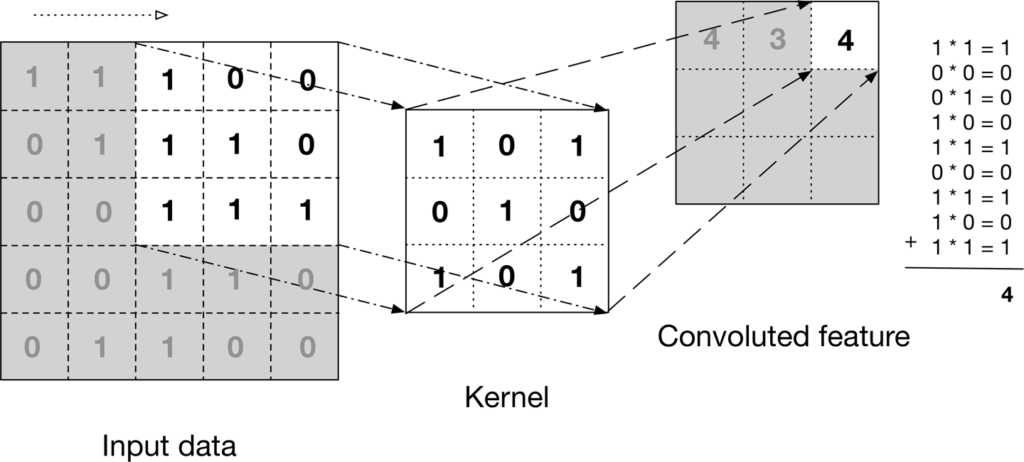
\includegraphics[width=0.45\textwidth]{The basic working of the convolutional layer.png}
\caption{The basic working of the convolutional layer.}
\label{fig:conv_example}
\end{figure}
Zero-padding is manually applied by extending the input with zeros around the border to preserve feature map size after convolution, which is crucial for deep architectures.

\begin{figure} [htbp]
    \centering
    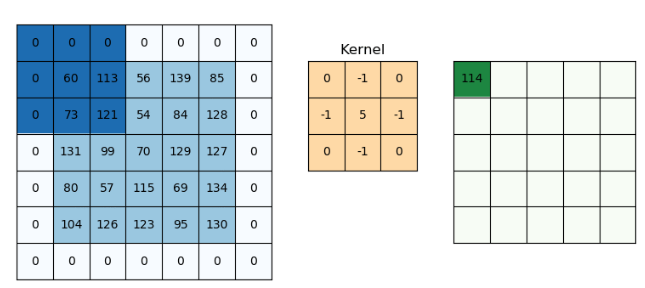
\includegraphics[width=0.75\linewidth]{Zero-padding.png}
    \caption{Example of Zero-padding }
    \label{fig:enter-label}
\end{figure}

\subsubsection{Pooling layer}

The pooling layer reduces the spatial dimensions of feature maps, helping to decrease computation and control overfitting. In this project, we implement \textbf{max pooling} using a $2 \times 2$ window with stride 2.

For input $X \in \mathbb{R}^{B \times C \times H \times W}$, the output $Y$ is given by:

\[
Y[b, c, i, j] = \max_{\substack{0 \leq u < 2 \\ 0 \leq v < 2}} X[b, c, 2i + u, 2j + v]
\]

This reduces the spatial size by half, while keeping the number of channels unchanged.

During backpropagation, the gradient is routed only through the max value in each region:

\[
\frac{\partial L}{\partial X[b, c, h, w]} =
\begin{cases}
\frac{\partial L}{\partial Y[b, c, i, j]} & \text{if } X[b, c, h, w] = Y[b, c, i, j] \\
0 & \text{otherwise}
\end{cases}
\]

\begin{figure}[htbp]
    \centering
    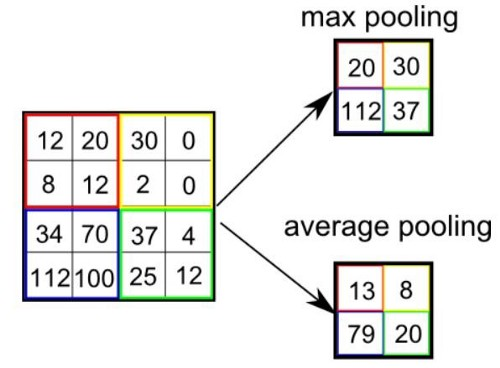
\includegraphics[width=0.5\linewidth]{pooling.png}
    \caption{Two types of pooling: max pooling and average pooling.}
    \label{fig:enter-label}
\end{figure}

\subsubsection{Flatten and Dense Layers}

After the convolution and pooling stages, the 3D feature maps are flattened into a 1D vector to be passed into the final classification layer.

Assume the output of the pooling layer has dimensions $(C, H, W)$, where $C$ is the number of channels, and $H$, $W$ are the spatial dimensions. The flatten operation rearranges this into a vector of size $C \times H \times W$.

The dense (fully connected) layer then computes a linear transformation followed by an activation function. For input vector $x$ and output size $D$ (e.g., 10 classes for digit classification), we compute:

\[
y_i = f\left( \sum_{j=1}^{C \cdot H \cdot W} w_{ij} \cdot x_j + b_i \right), \quad \text{for } i = 1, \dots, D
\]

where:
\begin{itemize}
  \item $w_{ij}$ is the weight from input $j$ to output $i$,
  \item $b_i$ is the bias term for class $i$,
  \item $f$ is an activation function (e.g., ReLU or softmax).
\end{itemize}
\begin{figure} [htbp]
    \centering
    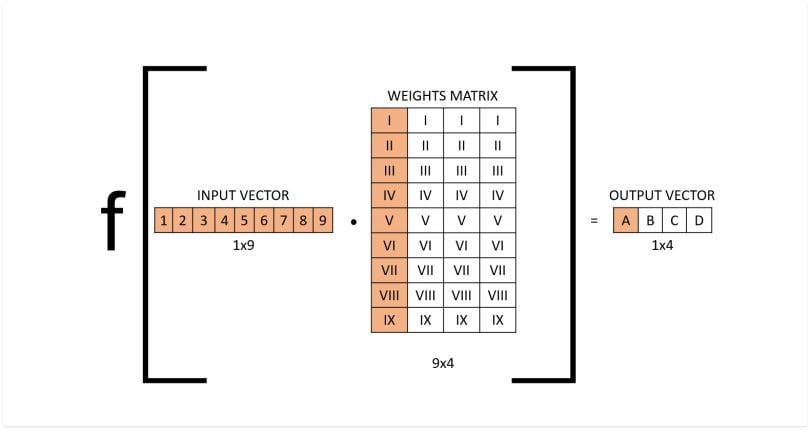
\includegraphics[width=0.75\linewidth]{fully.png}
    \caption{ the fully connected layer's input multiplied by the weights matrix to receive the output vector.}
    \label{fig:enter-label}
\end{figure}
Weights are initialized randomly within a small range, and biases are initialized to zero. All parameters are updated using gradients computed during backpropagation. The output represents raw scores for each class, which are later converted to probabilities using the softmax function.

\subsection{Activation Functions}

Activation functions introduce non-linearity into the model, enabling it to learn complex patterns beyond simple linear mappings. In our implementation, two common activation functions are used: \textbf{Sigmoid} and \textbf{ReLU (Rectified Linear Unit)}. These are applied element-wise on scalar values rather than tensors.

\subsubsection{Sigmoid Function}

The sigmoid function maps any real-valued input to a range between 0 and 1. It is defined as:

\[
\sigma(x) = \frac{1}{1 + e^{-x}}
\]

It is often used in binary classification or the final layer when we need probability output. However, in deeper layers, it may suffer from vanishing gradients.

\paragraph{Derivative:}

\[
\sigma'(x) = \sigma(x)(1 - \sigma(x))
\]

This is necessary during backpropagation to update weights.

\subsubsection{ReLU Function}

The ReLU function is one of the most widely used activation functions in deep learning. It is defined as:

\[
\text{ReLU}(x) = \max(0, x)
\]

This function simply outputs zero if the input is negative, otherwise it returns the input itself. ReLU is computationally efficient and helps avoid the vanishing gradient problem in deep networks.

\paragraph{Derivative:}

\[
\text{ReLU}'(x) =
\begin{cases}
1 & \text{if } x > 0 \\
0 & \text{otherwise}
\end{cases}
\]

ReLU is commonly applied after each convolution or dense layer (except the output layer), as it allows the network to learn piecewise linear mappings.


\subsection{Loss Function: Cross-Entropy}

In this project, we employ the \textbf{cross-entropy loss} function, which is widely used for multi-class classification tasks. The loss measures the distance between the predicted class probabilities and the actual class labels.

Let $\hat{y}_i$ be the predicted probability for class $i$, and $y_i$ be the ground truth label in one-hot encoded form (i.e., $y_i = 1$ if it is the correct class, else $0$). The loss for a single sample is computed as:

\[
L = -\sum_{i=1}^{K} y_i \log(\hat{y}_i)
\]

where $K$ is the number of classes (in our case, $K = 10$ for digit classification from 0 to 9).

For a batch of $N$ samples, the average cross-entropy loss is:

\[
L_{\text{batch}} = -\frac{1}{N} \sum_{n=1}^{N} \sum_{i=1}^{K} y_{n,i} \log(\hat{y}_{n,i})
\]

This function penalizes confident but incorrect predictions by producing a large loss. Conversely, it encourages high probability for the correct class.

In the training loop, gradients of the loss are computed manually and used to update the weights through backpropagation.

\section{Experiment and Result}
\subsection{Dataset}

The MNIST (Modified National Institute of Standards and Technology) dataset is a benchmark dataset in machine learning and computer vision, widely used for evaluating models on the task of handwritten digit recognition. It consists of grayscale images of handwritten digits ranging from 0 to 9.

\subsubsection{Dataset Description}

\begin{itemize}
    \item \text{Number of samples:} 70,000 images in total.
    \item \text{Training set:} 60,000 images.
    \item \text{Test set:} 10,000 images.
    \item \text{Image size:} Each image is $28 \times 28$ pixels, resulting in 784 input features.
    \item \text{Color channels:} Single channel (grayscale), pixel values range from 0 to 255.
    \item \text{Labels:} One of 10 classes (digits 0 through 9).
\end{itemize}

\subsubsection{Preprocessing}

Before training, each image is normalized by scaling pixel values to the range $[0, 1]$ by dividing by 255. No further augmentation or reshaping is performed, as the dataset is already standardized.

The MNIST dataset is particularly well-suited for testing classification models and understanding the performance of neural networks in recognizing patterns and features in visual data. Its relatively small size and well-labeled structure make it ideal for educational and experimental purposes.

In this project, MNIST is used as the primary dataset to evaluate the performance of a manually implemented Convolutional Neural Network (CNN) without relying on tensor libraries.

\subsubsection{Data Normalization}

To improve the stability and efficiency of the training process, the input images are normalized. Originally, each MNIST image contains pixel intensity values ranging from 0 to 255. These values are scaled to a range of $[0, 1]$ using min-max normalization:

\begin{equation}
x_{\text{norm}} = \frac{x}{255}
\end{equation}

Here, $x$ is the original pixel value, and $x_{\text{norm}}$ is the normalized pixel value.

\begin{itemize}
    \item Reduces the magnitude of input values, which helps in faster and more stable convergence during training.
    \item Ensures consistent input scale across all features, which is important for models using gradient-based optimization.
    \item Prevents issues like exploding gradients and improves generalization.
\end{itemize}

In this project, normalization is applied uniformly across the dataset before feeding the images into the convolutional layers.

\subsection{Result}

The performance of the neural network was evaluated by monitoring the loss during training and computing the final classification accuracy on the test set. The model was trained for 50 epochs, and the evolution of the loss is visualized in Figure~\ref{fig:loss_plot}. Table~\ref{tab:loss_summary} summarizes the loss values at selected epochs.

\begin{table}[!h]
\centering
\begin{tabular}{|c|c|}
\hline
\textbf{Epoch} & \textbf{Loss} \\
\hline
1  & 7.5486 \\
5  & 2.2210 \\
10 & 1.9577 \\
20 & 1.3747 \\
30 & 1.2078 \\
40 & 0.9962 \\
50 & 0.9073 \\
\hline
\end{tabular}
\vspace{0.5em}
\caption{Loss values at selected training epochs}
\label{tab:loss_summary}
\end{table}

\begin{figure}[!h]
    \centering
    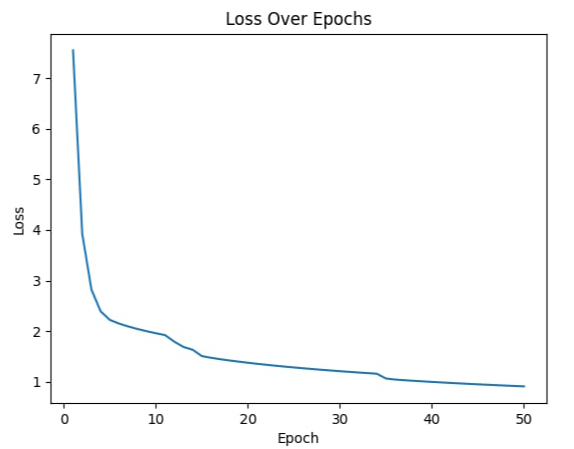
\includegraphics[width=0.6\textwidth]{loss_.png}
    \caption{Loss over training epochs}
    \label{fig:loss_plot}
\end{figure}

As shown in both the table and the figure, the training loss decreased rapidly during the first few epochs, from 7.5486 at epoch 1 to around 2.2 by epoch 5. After that, the loss continued to decline steadily, reaching 0.9073 at epoch 50, indicating effective learning and convergence of the model.

The final classification accuracy achieved by the network on the test set was \textbf{75\%}. This result suggests that while the model generalizes reasonably well, there is still room for improvement, possibly through hyperparameter tuning, more training data, or architectural enhancements.



\section{Conclusion}

Through 50 epochs of training, the model showed a significant reduction in loss, starting from a high initial value of 7.5486 and converging towards 0.9073 by the final epoch. This indicates that the network successfully learned from the training data and gradually minimized the error during prediction.

The training loss decreased rapidly in the first 10 epochs, followed by a slower but consistent improvement. This pattern is common in neural network training, where initial improvements are steep due to large gradients, and later stages focus on fine-tuning.

The final model achieved an accuracy of approximately 75\% on the evaluation set. While this suggests a reasonably good performance, there is still room for improvement. Potential enhancements could include tuning hyperparameters (e.g., learning rate, number of epochs), increasing model complexity, or applying regularization techniques to prevent overfitting.

Overall, the experiment demonstrates that the implemented neural network can learn meaningful representations and make accurate predictions, but further refinements are needed to push the performance closer to state-of-the-art benchmarks.

\section*{Acknowledgment}

We sincerely thank Assoc. Prof. Tran Giang Son for his insightful guidance and for proposing the minimalist challenge that inspired a deeper exploration of fundamental concepts.

\begin{thebibliography}{00}
\bibitem{lecun1998gradient} Y. LeCun, L. Bottou, Y. Bengio, and P. Haffner, "Gradient-based learning applied to document recognition," *Proceedings of the IEEE*, vol. 86, no. 11, pp. 2278–2324, 1998.

\bibitem{krizhevsky2012imagenet} A. Krizhevsky, I. Sutskever, and G. E. Hinton, "ImageNet classification with deep convolutional neural networks," in *Advances in Neural Information Processing Systems*, 2012, pp. 1097–1105.

\bibitem{goodfellow2016deep} I. Goodfellow, Y. Bengio, and A. Courville, *Deep Learning*, MIT Press, 2016.

\bibitem{dumoulin2016guide} V. Dumoulin and F. Visin, "A guide to convolution arithmetic for deep learning," arXiv preprint arXiv:1603.07285, 2016.

\bibitem{chollet2017deep} F. Chollet, *Deep Learning with Python*, Manning Publications, 2017.

\bibitem{bishop2006pattern} C. M. Bishop, *Pattern Recognition and Machine Learning*, Springer, 2006.

\bibitem{he2015delving} K. He, X. Zhang, S. Ren, and J. Sun, "Delving deep into rectifiers: Surpassing human-level performance on ImageNet classification," in *Proceedings of the IEEE ICCV*, 2015, pp. 1026–1034.

\bibitem{zhang2015understanding} C. Zhang, S. Bengio, M. Hardt, B. Recht, and O. Vinyals, "Understanding deep learning requires rethinking generalization," arXiv preprint arXiv:1611.03530, 2016.

\bibitem{simonyan2014very} K. Simonyan and A. Zisserman, "Very deep convolutional networks for large-scale image recognition," arXiv preprint arXiv:1409.1556, 2014.

\bibitem{szegedy2015going} C. Szegedy et al., "Going deeper with convolutions," in *Proceedings of the IEEE CVPR*, 2015, pp. 1–9.

\bibitem{kingma2014adam} D. P. Kingma and J. Ba, "Adam: A method for stochastic optimization," arXiv preprint arXiv:1412.6980, 2014.

\bibitem{nielsen2015neural} M. A. Nielsen, *Neural Networks and Deep Learning*, Determination Press, 2015.

\bibitem{lecun2015deep} Y. LeCun, Y. Bengio, and G. Hinton, "Deep learning," *Nature*, vol. 521, pp. 436–444, 2015.

\end{thebibliography}

\end{document}
